\subsection{Iterasi II: Desain}
\label{subsec:iter2_desain}

\subsubsection{Perangkat Keras}

Oleh karena prioritas utama adalah menentukan \textit{azimuth} posisi pengguna relatif terhadap layar, penempatan mikrofon diubah menjadi seperti yang terlihat pada \autoref{fig:desain_mic_2}. Dengan perubahan desain ini, pendekatan terhadap masalah TDOA berubah dari seperti yang tergambar pada \autoref{fig:tdoa_before} menjadi seperti yang tergambar pada \autoref{fig:tdoa_after1} dan \autoref{fig:tdoa_after2}. Selain itu, lebih banyak pasangan mikrofon yang dapat digunakan untuk memperkirakan \textit{azimuth} posisi pengguna relatif terhadap layar. Dengan demikian, terdapat enam parameter yang berpotensi sebagai masukan JST, yaitu dua nilai TDOA dari dua pasang mikrofon yang saling berdekatan dan empat nilai PtPAR dari empat pasang mikrofon yang saling berjauhan. Dua nilai PtPAR dari dua pasang mikrofon yang saling berdekatan dapat diabaikan karena perbedaan amplitudo sinyal yang tertangkap oleh sepasang mikrofon yang letaknya berdekatan tidak signifikan.

\begin{figure}[htp!]
\vskip 1em
  \begin{center}
    \subfigure[Tampak muka]
    {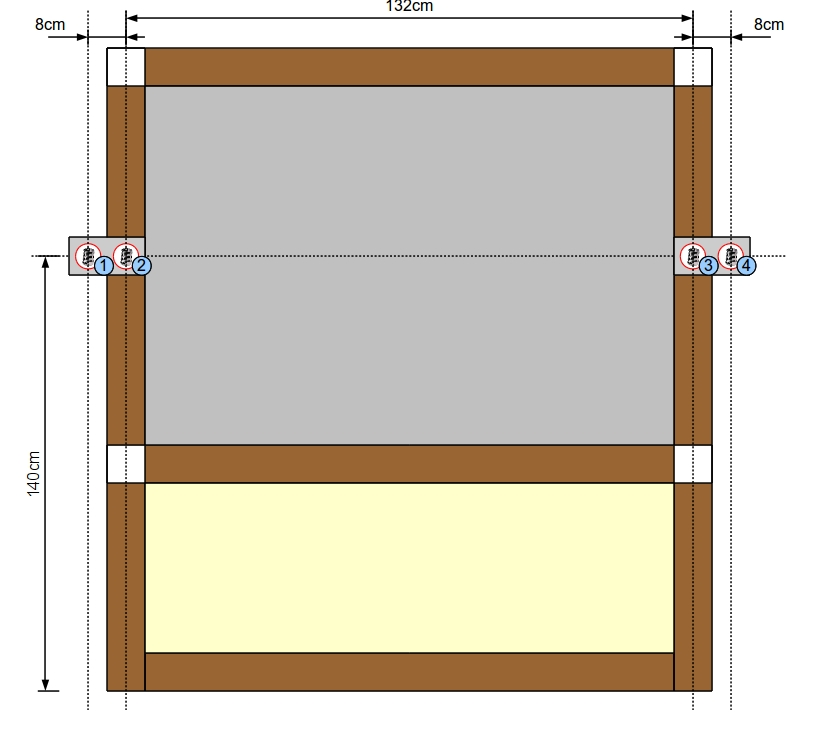
\includegraphics[scale=.5,keepaspectratio=true]{images/desain_mic_2a.jpg}
    \label{fig:desain_mic_2a}}
    \subfigure[Tampak atas]
    {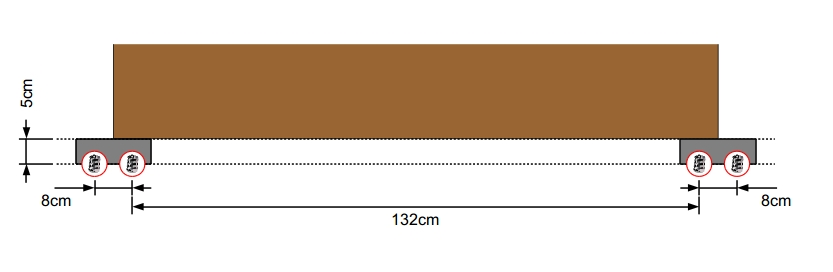
\includegraphics[scale=.5,keepaspectratio=true]{images/desain_mic_2b.jpg}
    \label{fig:desain_mic_2b}}
  \end{center}
  \caption[Perbaikan rancangan penempatan mikrofon]{Perbaikan rancangan penempatan mikrofon.}
  \label{fig:desain_mic_2}
  \vskip .5em
\end{figure}

\begin{figure}[htp!]
\vskip 1em
  \begin{center}
    \subfigure[]
    {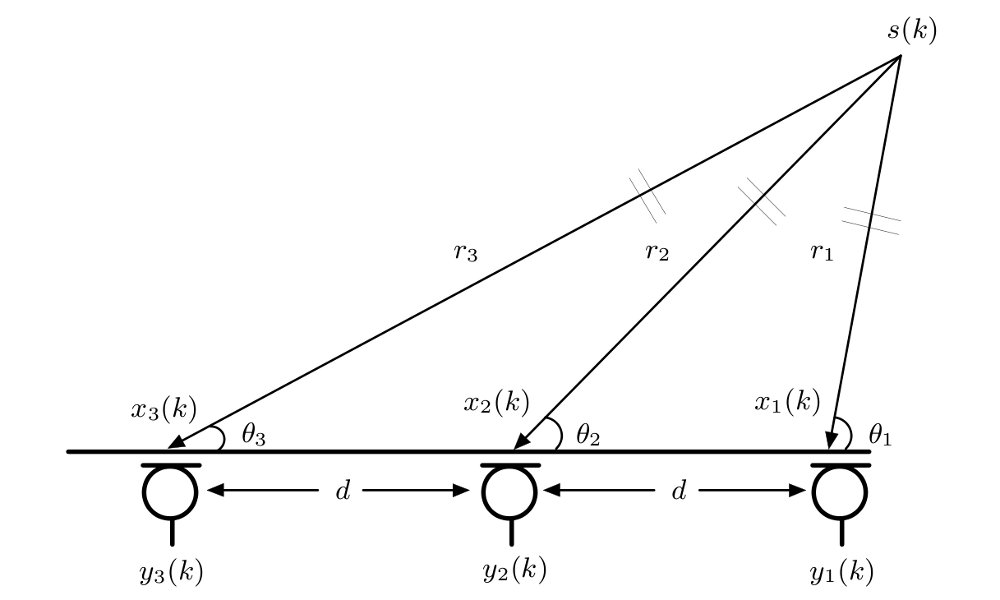
\includegraphics[scale=1.2,keepaspectratio=true]{images/tdoa_before.jpg}
    \label{fig:tdoa_before}}
    \subfigure[]
    {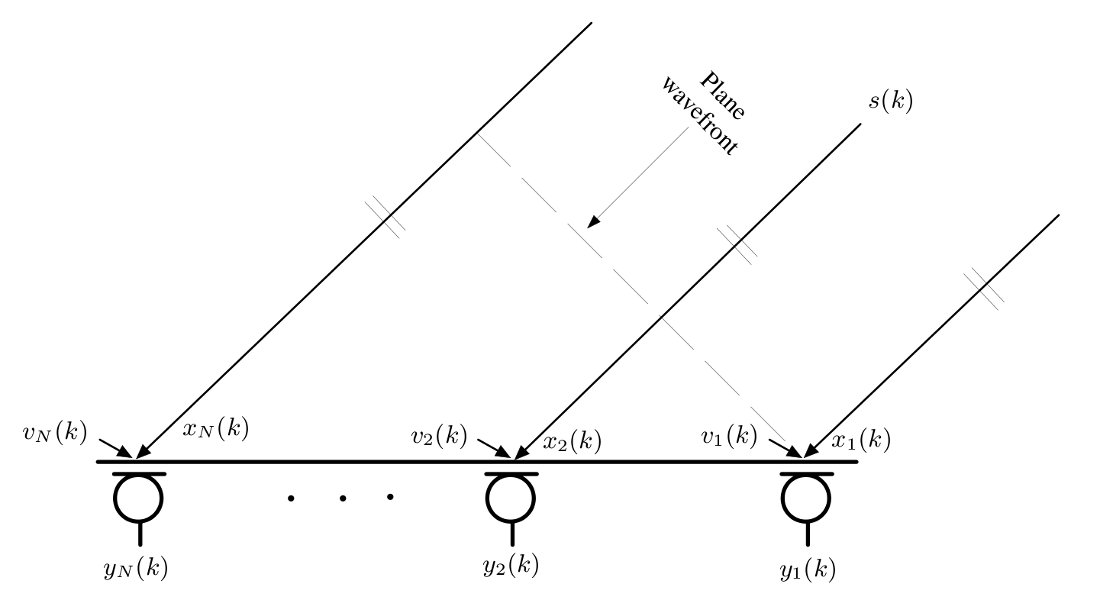
\includegraphics[scale=1.2,keepaspectratio=true]{images/tdoa_after1.jpg}
    \label{fig:tdoa_after1}}
    \subfigure[]
    {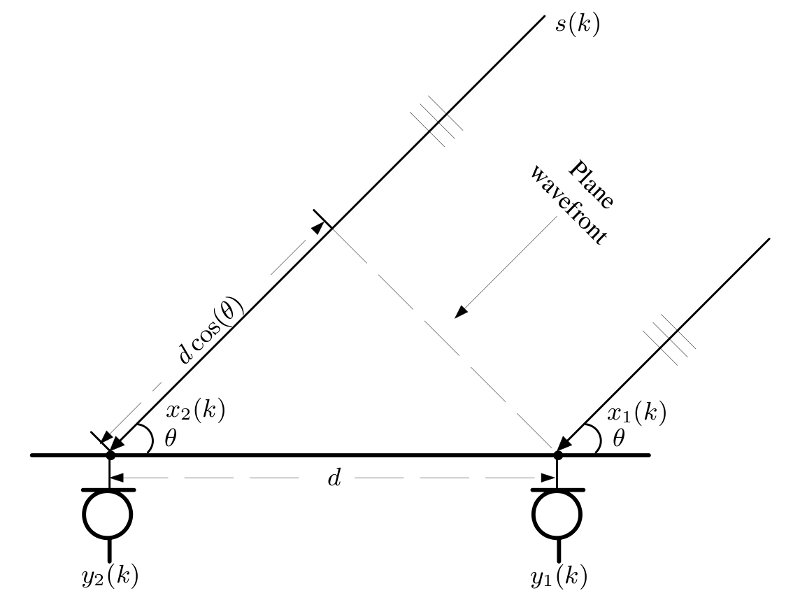
\includegraphics[scale=1.2,keepaspectratio=true]{images/tdoa_after2.jpg}
    \label{fig:tdoa_after2}}
  \end{center}
  \caption[Ilustrasi perubahan pendekatan masalah TDOA]{Ilustrasi perubahan pendekatan masalah TDOA \cite{benesty2008}.}
  \label{fig:tdoa_change}
  \vskip .5em
\end{figure}


\subsubsection{Pengambilan Data}

Jangkauan nilai koordinat sumber suara sama dengan yang digunakan sebelumnya (Iterasi I), yaitu $x = \{-50, 10, 70, 130, 190\}$, $y = \{60, 120, 180\}$, dan $z = -30$. Akan tetapi, titik-titik pengambilan data tersebut kemudian dibagi dalam kawasan-kawasan seperti yang ditunjukkan oleh \autoref{fig:floor_plan_2}. Oleh karena itu, apabila sebelumnya kemungkinan keluaran penentuan posisi pengguna adalah sebuah titik dalam koordinat Cartesian tiga dimensi yang relatif terhadap perangkat \textit{multitouch}, dengan penggunaan kawasan kemungkinan keluaran adalah sebuah sudut (\textit{azimuth}) yang relatif terhadap titik tengah perangkat \textit{multitouch}.

\begin{figure}[ht!]
\vskip 1em
\centering
 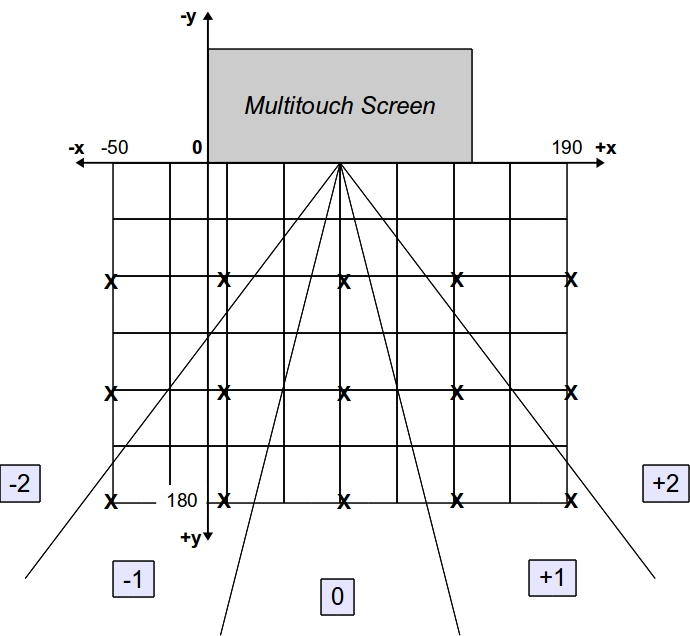
\includegraphics[scale=.5,keepaspectratio=true]{images/floor_plan_2.jpg}
 \caption[Perbaikan rancangan titik pengambilan data]{Perbaikan rancangan titik pengambilan data.}
 \label{fig:floor_plan_2}
\vskip .5em
\end{figure}

%%%%%%%%%%%%%%%%%%%%%%%%%%%%%%%%%%%%%%%%%%%%%%%%%%%%%%%%%%%%%%

\subsection{Iterasi II: Implementasi}

\subsubsection{Perangkat Keras}

Implementasi perbaikan rancangan penempatan mikrofon dapat dilihat pada \autoref{fig:desain_mic_2c1}. \autoref{fig:desain_mic_2c2} menunjukkan bagaimana mikrofon diletakkan dalam \textit{styrofoam} yang ditempelkan pada perangkat \textit{multitouch}.


\begin{figure}[ht!]
\vskip 1em
  \begin{center}
    \subfigure[]
    {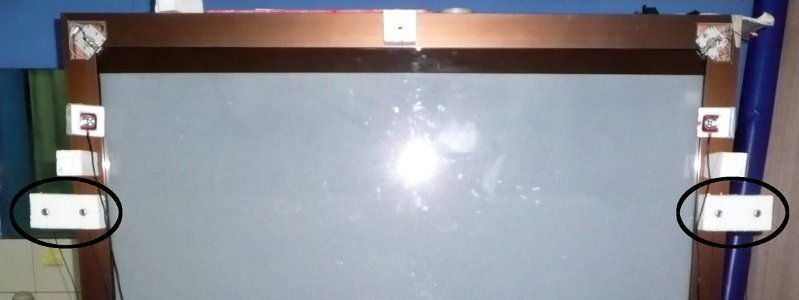
\includegraphics[width=.9\textwidth,keepaspectratio=true]{images/desain_mic_2c1.jpg}
    \label{fig:desain_mic_2c1}}
    \subfigure[]
    {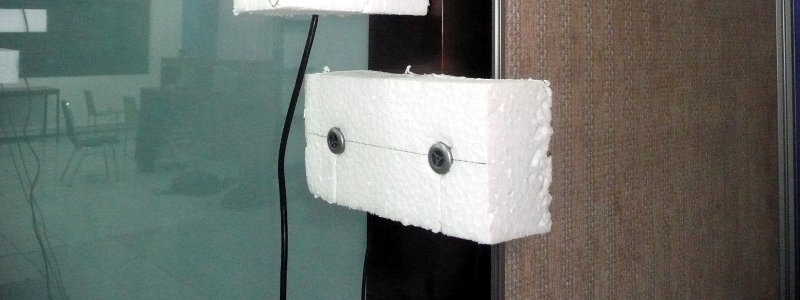
\includegraphics[width=.9\textwidth,keepaspectratio=true]{images/desain_mic_2c2.jpg}
    \label{fig:desain_mic_2c2}}
  \end{center}
  \caption[Foto implementasi perbaikan rancangan penempatan mikrofon]{Foto implementasi perbaikan rancangan penempatan mikrofon.}
  \label{fig:desain_mic_2c}
  \vskip .5em
\end{figure}

%%%%%%%%%%%%%%%%%%%%%%%%%%%%%%%%%%%%%%%%%%%%%%%%%%%%%%%%%%%%%%

\subsection{Iterasi II: Pengujian dan Evaluasi}

Dalam tahap ini, pengambilan data menggunakan empat file rekaman suara, yaitu FAN\_9B (ucapan kata "sembilan"), FAW\_7B (ucapan kata "tujuh"), MAF\_25A (ucapan frase "dua lima"), dan MSD\_5B (ucapan kata "lima"). Untuk memudahkan pembacaan grafik, jangkauan nilai koordinat $x = \{-50, 10, 70, 130, 190\}$ dan $y = \{60, 120, 180\}$ diubah menjadi $x = \{-4, -2, 0, 2, 4\}$ dan $y = \{-2, -4, -6\}$. 

Dari pengamatan terhadap empat set data, nilai parameter PtPAR cukup konsisten, sedangkan nilai parameter TDOA masih saja tidak konsisten. Dengan data tersebut, penentuan posisi pengguna diputuskan hanya akan menggunakan parameter PtPAR saja. Secara lebih spesifik, parameter PtPAR yang akan digunakan adalah parameter PtPAR mikrofon 1-3, 1-4, 2-3, dan 2-4.

Grafik TDOA dan PtPAR yang akan ditampilkan secara lengkap hanya set data FAN\_9B yang cukup merepresentasikan set data yang lain (\autoref{fig:2_fan_9b_tdoa_1} sampai dengan \autoref{fig:2_fan_9b_ptpar_3}). \autoref{fig:2_faw_7b_ptpar_1} dan \autoref{fig:2_faw_7b_ptpar_2} menunjukkan grafik PtPAR mikrofon 1-3, 1-4, 2-3, dan 2-4 dari set data FAW\_7B untuk memberikan gambaran lebih lanjut mengenai data latih dan data uji JST.

\begin{figure}[htp!]
\vskip 1em
  \begin{center}
    \subfigure[TDOA 1-2]
    {\fbox{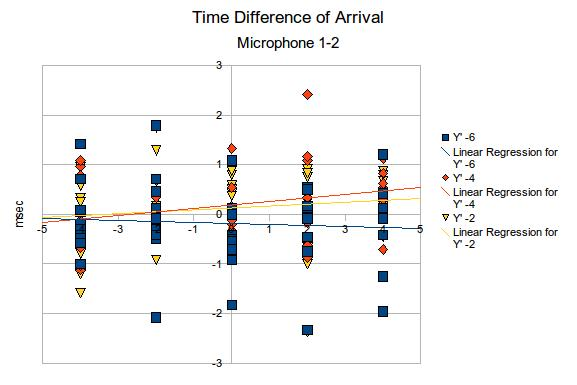
\includegraphics[scale=.55,keepaspectratio=true]{images/2_fan_9b_tdoa_12.jpg}
    \label{fig:2_fan_9b_tdoa_12}}}
    \subfigure[TDOA 3-4]
    {\fbox{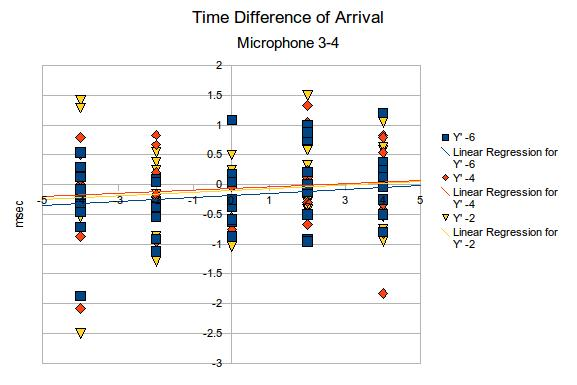
\includegraphics[scale=.55,keepaspectratio=true]{images/2_fan_9b_tdoa_34.jpg}
    \label{fig:2_fan_9b_tdoa_34}}}
  \end{center}
  \caption[Grafik TDOA dari set data FAN\_9B (1)]{Grafik TDOA dari set data FAN\_9B (1).}
  \label{fig:2_fan_9b_tdoa_1}
  \vskip .5em
\end{figure}

\begin{figure}[htp!]
\vskip 1em
  \begin{center}
    \subfigure[TDOA 1-3]
    {\fbox{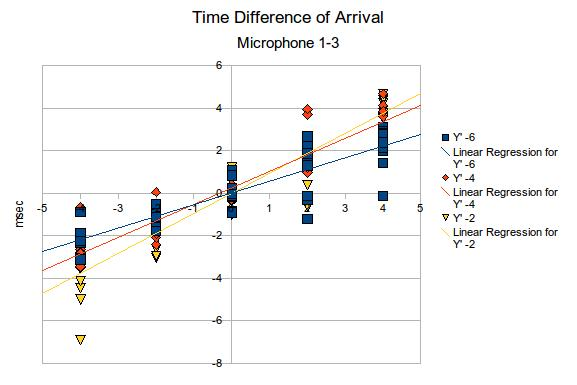
\includegraphics[scale=.55,keepaspectratio=true]{images/2_fan_9b_tdoa_13.jpg}
    \label{fig:2_fan_9b_tdoa_13}}}
    \subfigure[TDOA 1-4]
    {\fbox{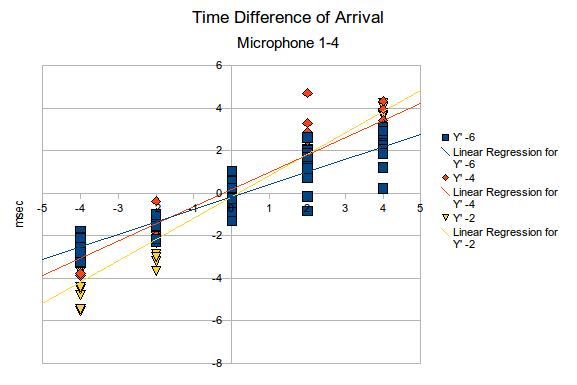
\includegraphics[scale=.55,keepaspectratio=true]{images/2_fan_9b_tdoa_14.jpg}
    \label{fig:2_fan_9b_tdoa_14}}}
  \end{center}
  \caption[Grafik TDOA dari set data FAN\_9B (2)]{Grafik TDOA dari set data FAN\_9B (2).}
  \label{fig:2_fan_9b_tdoa_2}
  \vskip .5em
\end{figure}

\begin{figure}[htp!]
\vskip 1em
  \begin{center}
    \subfigure[TDOA 2-3]
    {\fbox{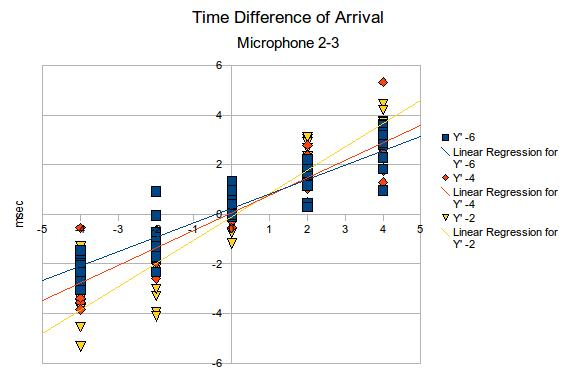
\includegraphics[scale=.55,keepaspectratio=true]{images/2_fan_9b_tdoa_23.jpg}
    \label{fig:2_fan_9b_tdoa_23}}}
    \subfigure[TDOA 2-4]
    {\fbox{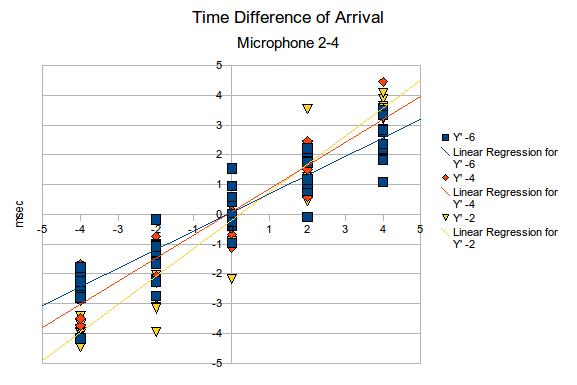
\includegraphics[scale=.55,keepaspectratio=true]{images/2_fan_9b_tdoa_24.jpg}
    \label{fig:2_fan_9b_tdoa_24}}}
  \end{center}
  \caption[Grafik TDOA dari set data FAN\_9B (3)]{Grafik TDOA dari set data FAN\_9B (3).}
  \label{fig:2_fan_9b_tdoa_3}
  \vskip .5em
\end{figure}

\begin{figure}[htp!]
\vskip 1em
  \begin{center}
    \subfigure[PtPAR 1-2]
    {\fbox{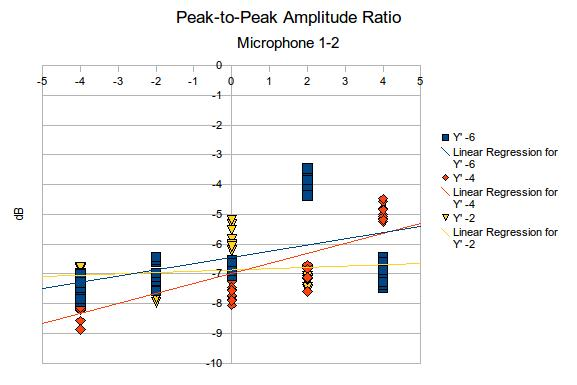
\includegraphics[scale=.55,keepaspectratio=true]{images/2_fan_9b_ptpar_12.jpg}
    \label{fig:2_fan_9b_ptpar_12}}}
    \subfigure[PtPAR 3-4]
    {\fbox{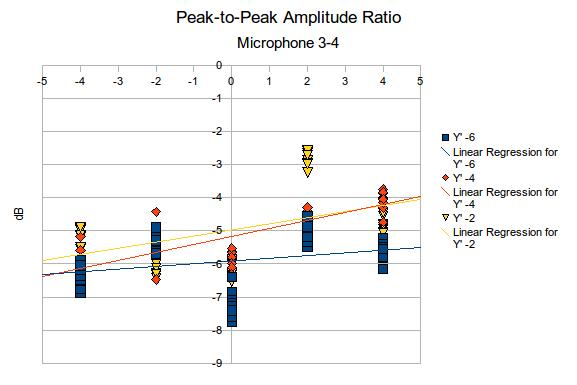
\includegraphics[scale=.55,keepaspectratio=true]{images/2_fan_9b_ptpar_34.jpg}
    \label{fig:2_fan_9b_ptpar_34}}}
  \end{center}
  \caption[Grafik PtPAR dari set data FAN\_9B (1)]{Grafik PtPAR dari set data FAN\_9B (1).}
  \label{fig:2_fan_9b_ptpar_1}
  \vskip .5em
\end{figure}

\begin{figure}[htp!]
\vskip 1em
  \begin{center}
    \subfigure[PtPAR 1-3]
    {\fbox{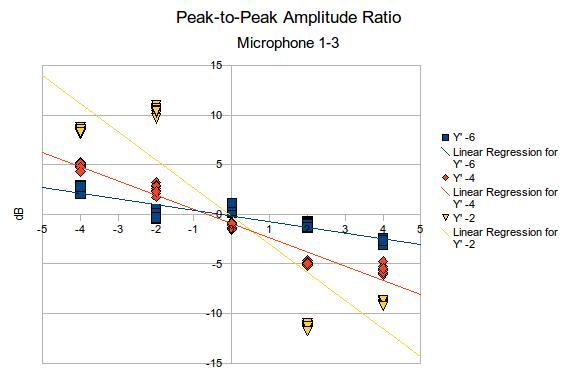
\includegraphics[scale=.55,keepaspectratio=true]{images/2_fan_9b_ptpar_13.jpg}
    \label{fig:2_fan_9b_ptpar_13}}}
    \subfigure[PtPAR 1-4]
    {\fbox{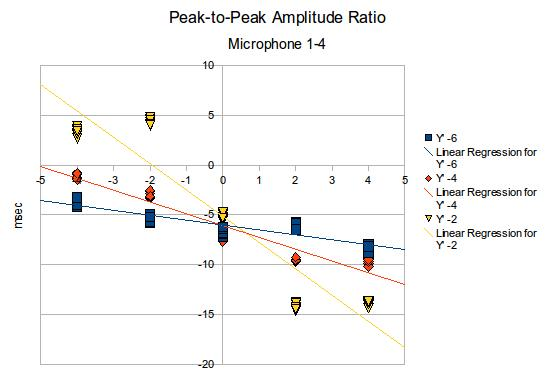
\includegraphics[scale=.55,keepaspectratio=true]{images/2_fan_9b_ptpar_14.jpg}
    \label{fig:2_fan_9b_ptpar_14}}}
  \end{center}
  \caption[Grafik PtPAR dari set data FAN\_9B (2)]{Grafik PtPAR dari set data FAN\_9B (2).}
  \label{fig:2_fan_9b_ptpar_2}
  \vskip .5em
\end{figure}

\begin{figure}[htp!]
\vskip 1em
  \begin{center}
    \subfigure[PtPAR 2-3]
    {\fbox{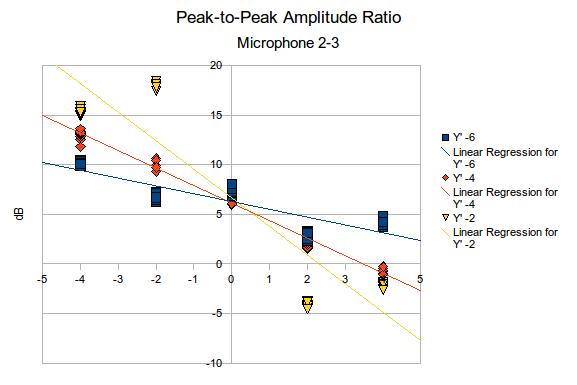
\includegraphics[scale=.55,keepaspectratio=true]{images/2_fan_9b_ptpar_23.jpg}
    \label{fig:2_fan_9b_ptpar_23}}}
    \subfigure[PtPAR 2-4]
    {\fbox{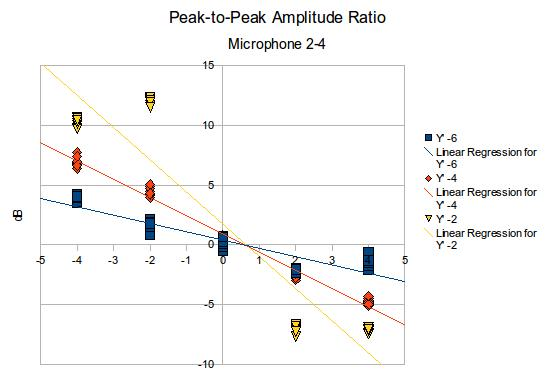
\includegraphics[scale=.55,keepaspectratio=true]{images/2_fan_9b_ptpar_24.jpg}
    \label{fig:2_fan_9b_ptpar_24}}}
  \end{center}
  \caption[Grafik PtPAR dari set data FAN\_9B (3)]{Grafik PtPAR dari set data FAN\_9B (3).}
  \label{fig:2_fan_9b_ptpar_3}
  \vskip .5em
\end{figure}

\begin{figure}[htp!]
\vskip 1em
  \begin{center}
    \subfigure[PtPAR 1-3]
    {\fbox{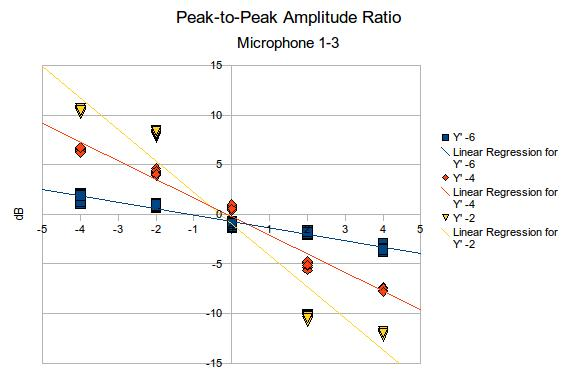
\includegraphics[scale=.55,keepaspectratio=true]{images/2_faw_7b_ptpar_13.jpg}
    \label{fig:2_faw_7b_ptpar_13}}}
    \subfigure[PtPAR 1-4]
    {\fbox{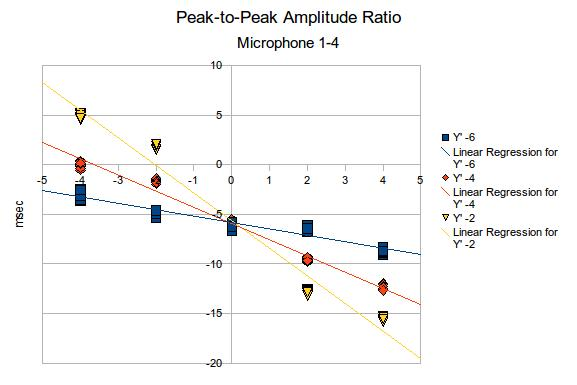
\includegraphics[scale=.55,keepaspectratio=true]{images/2_faw_7b_ptpar_14.jpg}
    \label{fig:2_faw_7b_ptpar_14}}}
  \end{center}
  \caption[Grafik PtPAR dari set data FAW\_7B (1)]{Grafik PtPAR dari set data FAW\_7B (1).}
  \label{fig:2_faw_7b_ptpar_1}
  \vskip .5em
\end{figure}

\begin{figure}[htp!]
\vskip 1em
  \begin{center}
    \subfigure[PtPAR 2-3]
    {\fbox{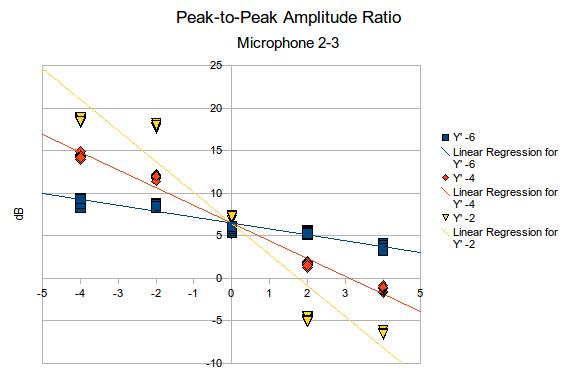
\includegraphics[scale=.55,keepaspectratio=true]{images/2_faw_7b_ptpar_23.jpg}
    \label{fig:2_faw_7b_ptpar_23}}}
    \subfigure[PtPAR 2-4]
    {\fbox{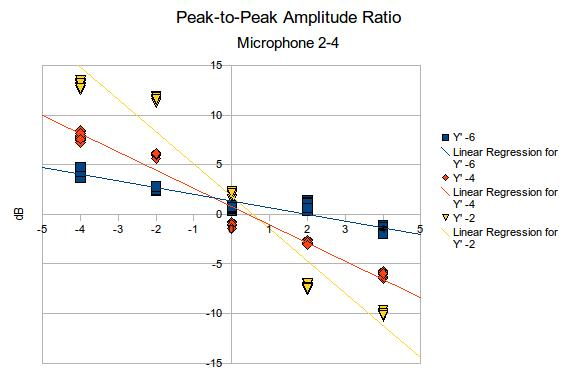
\includegraphics[scale=.55,keepaspectratio=true]{images/2_faw_7b_ptpar_24.jpg}
    \label{fig:2_faw_7b_ptpar_24}}}
  \end{center}
  \caption[Grafik PtPAR dari set data FAW\_7B (2)]{Grafik PtPAR dari set data FAW\_7B (2).}
  \label{fig:2_faw_7b_ptpar_2}
  \vskip .5em
\end{figure}
